For GASAL2 to work correctly, all data fields in the \texttt{gasal\_gpu\_storage\_t} structure must have their sizes specified at initialisation. This is problematic with BWA-MEM because sizes cannot be inferred beforehand. Even if we process a pack of 4000 reads, each of them have an unpredictable number of seeds. Furthermore, for each seed, the length of the query and target sequences are unknown. We show a schematic view for this problem on Figure~\ref{fig:cpu-gpu-batches}. The GPU accelerated BWA-MEM align the sequences in packs that are selected by the CPU. This pack is then split into muliple batches of sequences, each batch being processed by a CUDA stream. The figure shows two packs of 3 reads each (note the read numbers on the left, Q1 to Q6). For each read, there can be different number of seeds. The pack is distributed evenly between CUDA streams in GPU batches. Reads of the same colour are processed by the same GPU batch. This is difficult to show with a few number of sequences like here (for the first sequence pack, reads Q1 and Q2 are in the same GPU batch and read Q3 is in another GPU batch), but for example, a pack of 4000 sequences is split into 4 GPU batches of 1000 sequences each, each assigned to one CUDA stream. After each stream has been given its GPU batch to process, the seeding phase runs for each read, and multiple seeds are found. For each seed, the left and right parts of the alignment are copied onto the GPU memory and the kernel runs to compute the alignment. Alignments of the same colour are processed in the same GPU batch, so in the same CUDA stream. For example, if we have 2 CUDA streams, all seeds for Q4 are extended by Stream \#1, then all seeds from Q5 are processed by Stream \#2, then Q6 seeds are processed by Stream \#1 if we assume it has finished when Stream \#2 was computing. We can see that the total number of alignment is different depending on the number of seeds, and each alignment has its own left and right lengths.

\begin{figure}[h!]
	\centering
	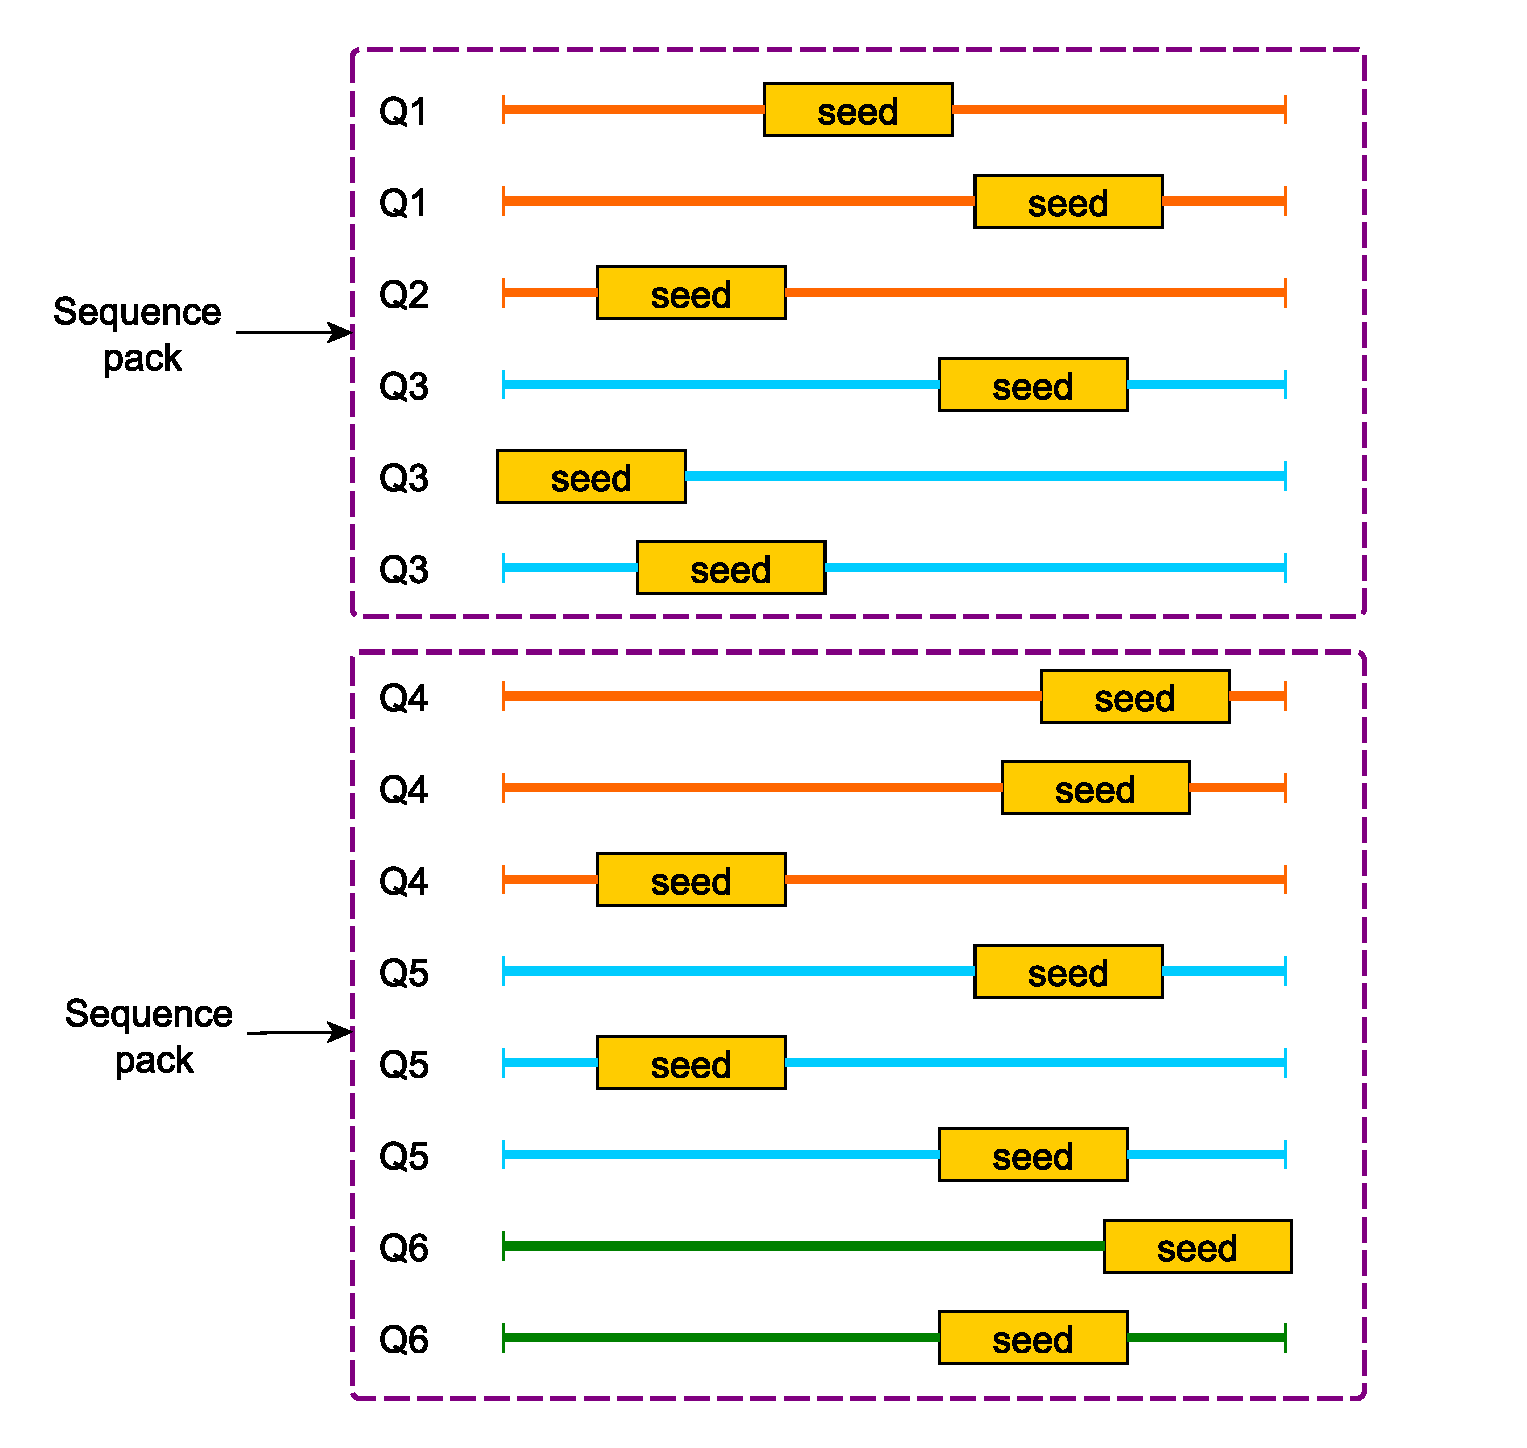
\includegraphics[width=1\linewidth]{cpu-gpu-batches}
	\caption{Representation of alignment distribution in sequences packs across GPU batches.}
	\label{fig:cpu-gpu-batches}
\end{figure}


We would need some automatic resizing whenever the initial size is insufficient.
For a given data set, during testing phase, we can estimate an upper bound. But this is not a good approach since we have to allocate much more memory than actually required.

In this section we will review the solutions we implemented. A simple approach was adopted for all the arrays carrying metadata for the sequences. We chose a more refined approach for the fields bearing the actual sequences to minimise overhead caused by reallocation.

\subsection{Memory reallocation for arrays fields}

A large number of fields in the \verb|gasal_gpu_storage_t| are containing information about the sequences. These fields are arrays of length equal to the number of sequences. As such, they do not store a very large amount of data, and their separation is clear (each slot of the array is holding information about one single sequence). For example, we need to store the length of each query and target, the offset of each each query and target, and so on. These fields are first allocated on host side, then they are copied onto the device, so they are allocated with \verb|CudaHostAlloc|. Since there are a large number of fields and they do not represent a major part of memory allocation, we decided to implement a simple realloc feature for all such fields. This function is displayed on listing~\ref{lst:cudarealloc}. Note that on the \verb|gasal_gpu_storage_t| shown on Listing~\ref{lst:gpu_storage}, all fields do not have the same type: some are of type \verb|uint32_t|, others are \verb|uint8_t|, and so on. We made a simple use of C++ template to adapt this function to multiple types. It allocates a new memory area, copies the content of the former area, and frees it. It returns a pointer to the newly allocated area in memory filled with the previous data. This re-allocator is called by a larger function resizing all the necessary fields when the number of sequences filled exceeds the number of maximum sequences the data structure can hold.

\begin{listing}[h!]
	\begin{minted}[frame=lines,
	framesep=2mm,
	baselinestretch=1.2,
	fontsize=\footnotesize,
	linenos,
	breaklines,
	frame=single]{C++}
// Function for general resizing
template <typename T>
T* cudaHostRealloc(void *source, int new_size, int old_size) 
{
	cudaError_t err;
	T* destination = NULL;
	if (new_size < old_size)
	{
		fprintf(stderr, "[GASAL ERROR] cudoHostRealloc: invalid sizes. New size < old size (%d < %d)", new_size, old_size);
		exit(EXIT_FAILURE);
	}
	CHECKCUDAERROR(cudaHostAlloc(&destination, new_size * sizeof(T), cudaHostAllocMapped));
	CHECKCUDAERROR(cudaMemcpy(destination, source, old_size * sizeof(T), cudaMemcpyHostToHost));
	CHECKCUDAERROR(cudaFreeHost(source));
	return destination;
};
	\end{minted}
	\caption{Reallocation function for CUDA allocated fields.}
	\label{lst:cudarealloc}
\end{listing}

The user of the library must take care of the sequence count and run the reallocator when needed. Once the fields are reallocated to a bigger memory area, they keep their new size, so they don't need to be re-allocated until the next time the new maximum capacity is exceeded. The library keeps track of size of the array and current number of sequences filled in it. 

We chose a different approach for the arrays that hold actual sequences because they are much bigger and reallocation is time expensive.

\subsection{Extensible data structure for sequences}

Using the same reallocation for the sequences could have been possible, but unpractical. In fact, these memory allocations and frees are costly in time. While this is reasonable for smaller arrays having only 4-bytes elements (like \verb|uint32_t|), it takes too much time with the sequences arrays. In the data structure, there are two fields to store the query sequences and the target sequences respectively. Each field is a single array and all sequences are put some following others in this array. If a batch has 1000 reads, there may be 10 000 to even 100 000 seeds for the whole batch, making it up to 200 000 alignments to performed (most seeds needing both left and right extension). Each base being stored in one byte, making them query and target arrays 20 to 30 times larger than the other arrays for sequence lengths, sequence offsets, or other information.

Due to this issue, we designed a structure of linked list to allocate more memory progressively without needing to move around already existing data. This structure shown on Listing~\ref{lst:extensiblehostbatch} starts with a single element and each of them carries some metadata about its content size to ensure correct filling. It stores:

\begin{itemize}
	\item the sequences, butted together, in the field \verb|*data|,
	\item how many bytes are already stored, in field \verb|data_size|,
	\item the total size available in bytes, in the field \verb|page_size|,
	\item the data \verb|offset|, which is equal to the data size of the previous element of the linked list,
	\item A flag telling is the structure can store new data or not, \verb|is_locked|, set to 0 or 1,
	\item and of course, as for all linked list, a pointer to the next element.
\end{itemize}

\begin{listing}[h!]
	\begin{minted}[frame=lines,
	framesep=2mm,
	baselinestretch=1.2,
	fontsize=\footnotesize,
	linenos,
	breaklines,
	frame=single]{C++}
struct host_batch{
	uint8_t *data;
	uint32_t page_size;
	uint32_t data_size;
	uint32_t offset;
	int is_locked;
	struct host_batch* next;
};
typedef struct host_batch host_batch_t;
	\end{minted}
\caption{The linked list structure for sequences on host.}
\label{lst:extensiblehostbatch}
\end{listing}

The sequences are filled by a dedicated function from GASAL2 that takes care of allocating more memory if needed. This function takes as input the sequence to add, the storage structure, and if it is a query or target sequence to fill, Algorithm~\ref{algo:extensiblefunction} shows the pseudocode of the function. We represent the fields belonging to an element with the symbol $\rhd$, similar to the symbol \verb|->| used in C++ to access the field belonging to a pointer of a structure.


\begin{algorithm}[h!]
	\caption{Behaviour of the sequence filler function}
	\label{algo:extensiblefunction}
	\begin{algorithmic}[1] % The number tells where the line numbering should start
		\Function{Fills one sequence in an linked list }{$gasal\_gpu\_storage\_t$, $seq$, $seq_length$, $seq_offset$, $data\_source$}
		
		\State Select query or target linked list from $data\_source$
		\State Select first non-locked linked-list element, $~e$
		\State Compute padding length $padding\_length$
		\State $total\_length \leftarrow padding\_length + seq\_length$
		
		\If{$e$ is the last element \textbf{and} $total\_length \geqslant e\rhd page\_size - e\rhd data\_size$}
			\State Create new element twice as big
			\State Append it to the last element $e$
			\State Select last element (newly added) of the linked list, define it as $e$
		\EndIf
		
		\If{$e$ is not the last element \textbf{and} $total\_length \geqslant e\rhd page\_size - e\rhd data\_size$}
			\State $e\rhd next\rhd offset \leftarrow e\rhd offset + e\rhd data\_size $
			\State Mark $e$ as locked
			\State Select next element $e\rhd next$ of the linked list, define it as $e$
		\EndIf
		
		%\If{$total\_length \leqslant e\rhd page\_size - e\rhd data\_size$}
			\State Store the sequence in $e\rhd data$ add the padding
			\State $e\rhd data\_size \leftarrow e\rhd data\_size + total\_size$
		%\EndIf
		
		
		\Return $offset$
		\EndFunction
		
	\end{algorithmic}
\end{algorithm}

In the beginning, the first non-locked element is selected. Then the algorithm operates in three main steps. 

\begin{enumerate}
	\item First (line 6), it checks if the selected element is the end of the linked list, and if there is not enough space in it. If so, the only solution is to create a new element to append at the end of the linked list.
	\item Then (line 11), it checks if the current element is full and if there are more elements down the linked list. This happens when the linked list has created new elements during previous fillings and kernel launches. We already selected the first non-locked element, so if it is full, we simply jumps to the next one, and lock the previous one so that we don't try to fill it anymore.
	\item At this point (line 16), we have reached an element which have enough free space for the sequence:
	\begin{itemize}
	    \item if we had an element available from the beginning, we reach this point without going through the previous \verb|if|.
	    \item if the last non-locked element was full, we locked it and jumped to the next one, so we reached a non-full element,
	    \item if we were at the end of the list, we created a new element and jumped to it.
    \end{itemize}
    We can now fill it with the sequence and its offset.
\end{enumerate}

In the end, the function returns the current offset, corresponding to the total number of bytes present in the linked list, which is needed to continue the filling for the next sequence.

Globally, we have a linked list of structures filled by full sequences. We do not split the sequences between two elements. Therefore, each element is not filled up to its maximum capacity, leaving an area smaller than a sequence length unused.

When copying the batches onto the device, all elements are processed using \verb|CudaMemCpy|. The size to copy is directly given by the field \verb|data_size|. At this moment, all the elements in the linked list are set as "non-locked". This way, they can be re-used for future launches. The linked list can only grow in size to minimise the possibility of having to do another allocation later on. This is why we implemented this "locked" flag to get the information if the element has been filled for the current batch, to know where to start filling up.

All in all, this allocation scheme allows to get more memory space without moving around already existing data by re-using all the previously created memory chunks in the linked list, and creating bigger elements. Since we would like to keep the number of allocations to a minimum, we allocate bigger memory chunks each time it is needed. The more allocations are done, the bigger they are: it becomes less and less likely to trigger a new allocation as we grow in size.

%\vspace{0.1\textheight}
\section*{Wrap-up}
In this chapter, we reviewed all the modifications and new implementation we carried out to successfully integrate GASAL2 in BWA-MEM. We started from a demonstrator (GASE-GASAL2) already processing in pack of reads, and we ported it to C++ to run it with the newer version of GASAL2. We created a CUDA kernel that replicates the behaviour of the original C function in BWA-MEM. We integrated the library with our "seed-only" paradigm to tackle the issue of processing both sides of the extension in parallel. This created its own issues with score synchronisation between left and right sides, and we addressed this problem by keeping track of the number of alignments to guarantee correctness of the score. The memory management is now done with the help of memory reallocation for small arrays and using linked list of elements for the actual sequences arrays to minimise the number of time expensive memory reallocation operations. Finally, we tested this implementation in our hardware with a sample data set, that we will present in the next chapter.


